\chapter{Cloud Security with Honeypots}

\section{Introduction}

\todo{Daten sammeln mit T-Pot fuer Auswertungen, etc.. Bezug auf bisherige Arbeiten nehmen}

\citet{Nithin2012}

\citet{Kelly2021}

\section{HeiCloud}

\citet{urz2021} offers a \enquote{\ac{iaas} specially tailored for higher education and research institutions}.
Key idea is that it supplies 

\cite{heicloud2021}

\begin{itemize}
    \item IaaS for science
    \item Freely manage IT resources by yourself
    \item Stable and fast connection
    \item High availability
    \item High security standards
    \item High scalability
    \item Open Source
    \item Freely selectable VM operating systems
    \item Transparent accounting
    \item Available in the German Research Network
\end{itemize}

\section{T-Pot}

T-Pot is a hollistic honeypot approach to capture recent cyber attacks. 
In conjucntion with a
\todo{Zusammenfassung tpot, funktionalitaet etc.}

\todo{Quelle jedes Honeypots hinzufügen}
\begin{itemize}
    \item adbhoney \cite{adbhoney2021}
    \item ciscoasa \cite{cymmetria2018}
    \item citrixhoneypot \cite{citrixhoneypot2020}
    \item conpot \cite{conpot2021}
    \item cowrie \cite{cowire2021}
    \item ddospot \cite{ddosspot2021}
    \item dicompot \cite{dicompot2021}
    \item dionaea \cite{dionaea2021}
    \item elasticpot \cite{elasticpot2021}
    \item endlessh \cite{endlessh2021}
    \item glutton \cite{glutton2021}
    \item heralding \cite{heralding2021}
    \item hellpot \cite{hellpot2021}
    \item honeypy \cite{honeysap2021}
    \item honeysap \cite{honeysap2021}
    \item honeytrap \cite{honeytrap2021}
    \item ipphoney \cite{ipphoney2021}
    \item mailoney
    \item medpot \cite{medpot2021}
    \item rdpy \cite{rdpy2021}
    \item redishoneypot
    \item snare \cite{snare2021}
    \item tanner \cite{tanner2021}
\end{itemize}

\begin{table}[h]
    \centering
    \caption{Overview of all available honeypots of T-Pot}
    \begin{tabularx}{\linewidth}{l|l|l}
        \toprule
        \textbf{Honeypot}                                 & \textbf{Description} & \textbf{Port} \\
        \hline
        adbhoney                                 &             &      \\
        ciscoasa \cite{cymmetria2018}            &             &      \\
        citrixhoneypot \cite{citrixhoneypot2020} &             &      \\
        conpot \cite{conpot2021}                 &             &      \\
        cowrie \cite{cowire2021}                 &             &      \\
        ddospot \cite{ddosspot2021}              &             &      \\
        dicompot \cite{dicompot2021}             &             &      \\
        dionaea \cite{dionaea2021}               &             &      \\
        elasticpot \cite{elasticpot2021}         &             &      \\
        endlessh \cite{endlessh2021}             &             &      \\
        glutton \cite{glutton2021}               &             &      \\
        heralding \cite{heralding2021}           &             &      \\
        hellpot \cite{hellpot2021}               &             &      \\
        honeypy \cite{honeysap2021}              &             &      \\
        honeysap \cite{honeysap2021}             &             &      \\
        honeytrap \cite{honeytrap2021}           &             &      \\
        ipphoney \cite{ipphoney2021}             &             &      \\
        mailoney                                 &             &      \\
        medpot \cite{medpot2021}                 &             &      \\
        rdpy \cite{rdpy2021}                     &             &      \\
        redishoneypot                            &             &      \\
        snare \cite{snare2021}                   &             &      \\
        tanner \cite{tanner2021}                 &             &      \\
        \bottomrule
    \end{tabularx}
    \label{tab:overview-honeypots}
\end{table}

In addition, T-Pot integrates following tools to investigate and handle network traffic:

\begin{itemize}
    \item Cockpit
    \item Cyberchef
    \item ELK stack
    \item Elasticsearch head
    \item Fatt
    \item Spiderfoot
    \item Suricata
\end{itemize}

\todo{Übersicht zu Tpot, eigene Grafik}


\begin{sidewaysfigure}[h]
    \centering
    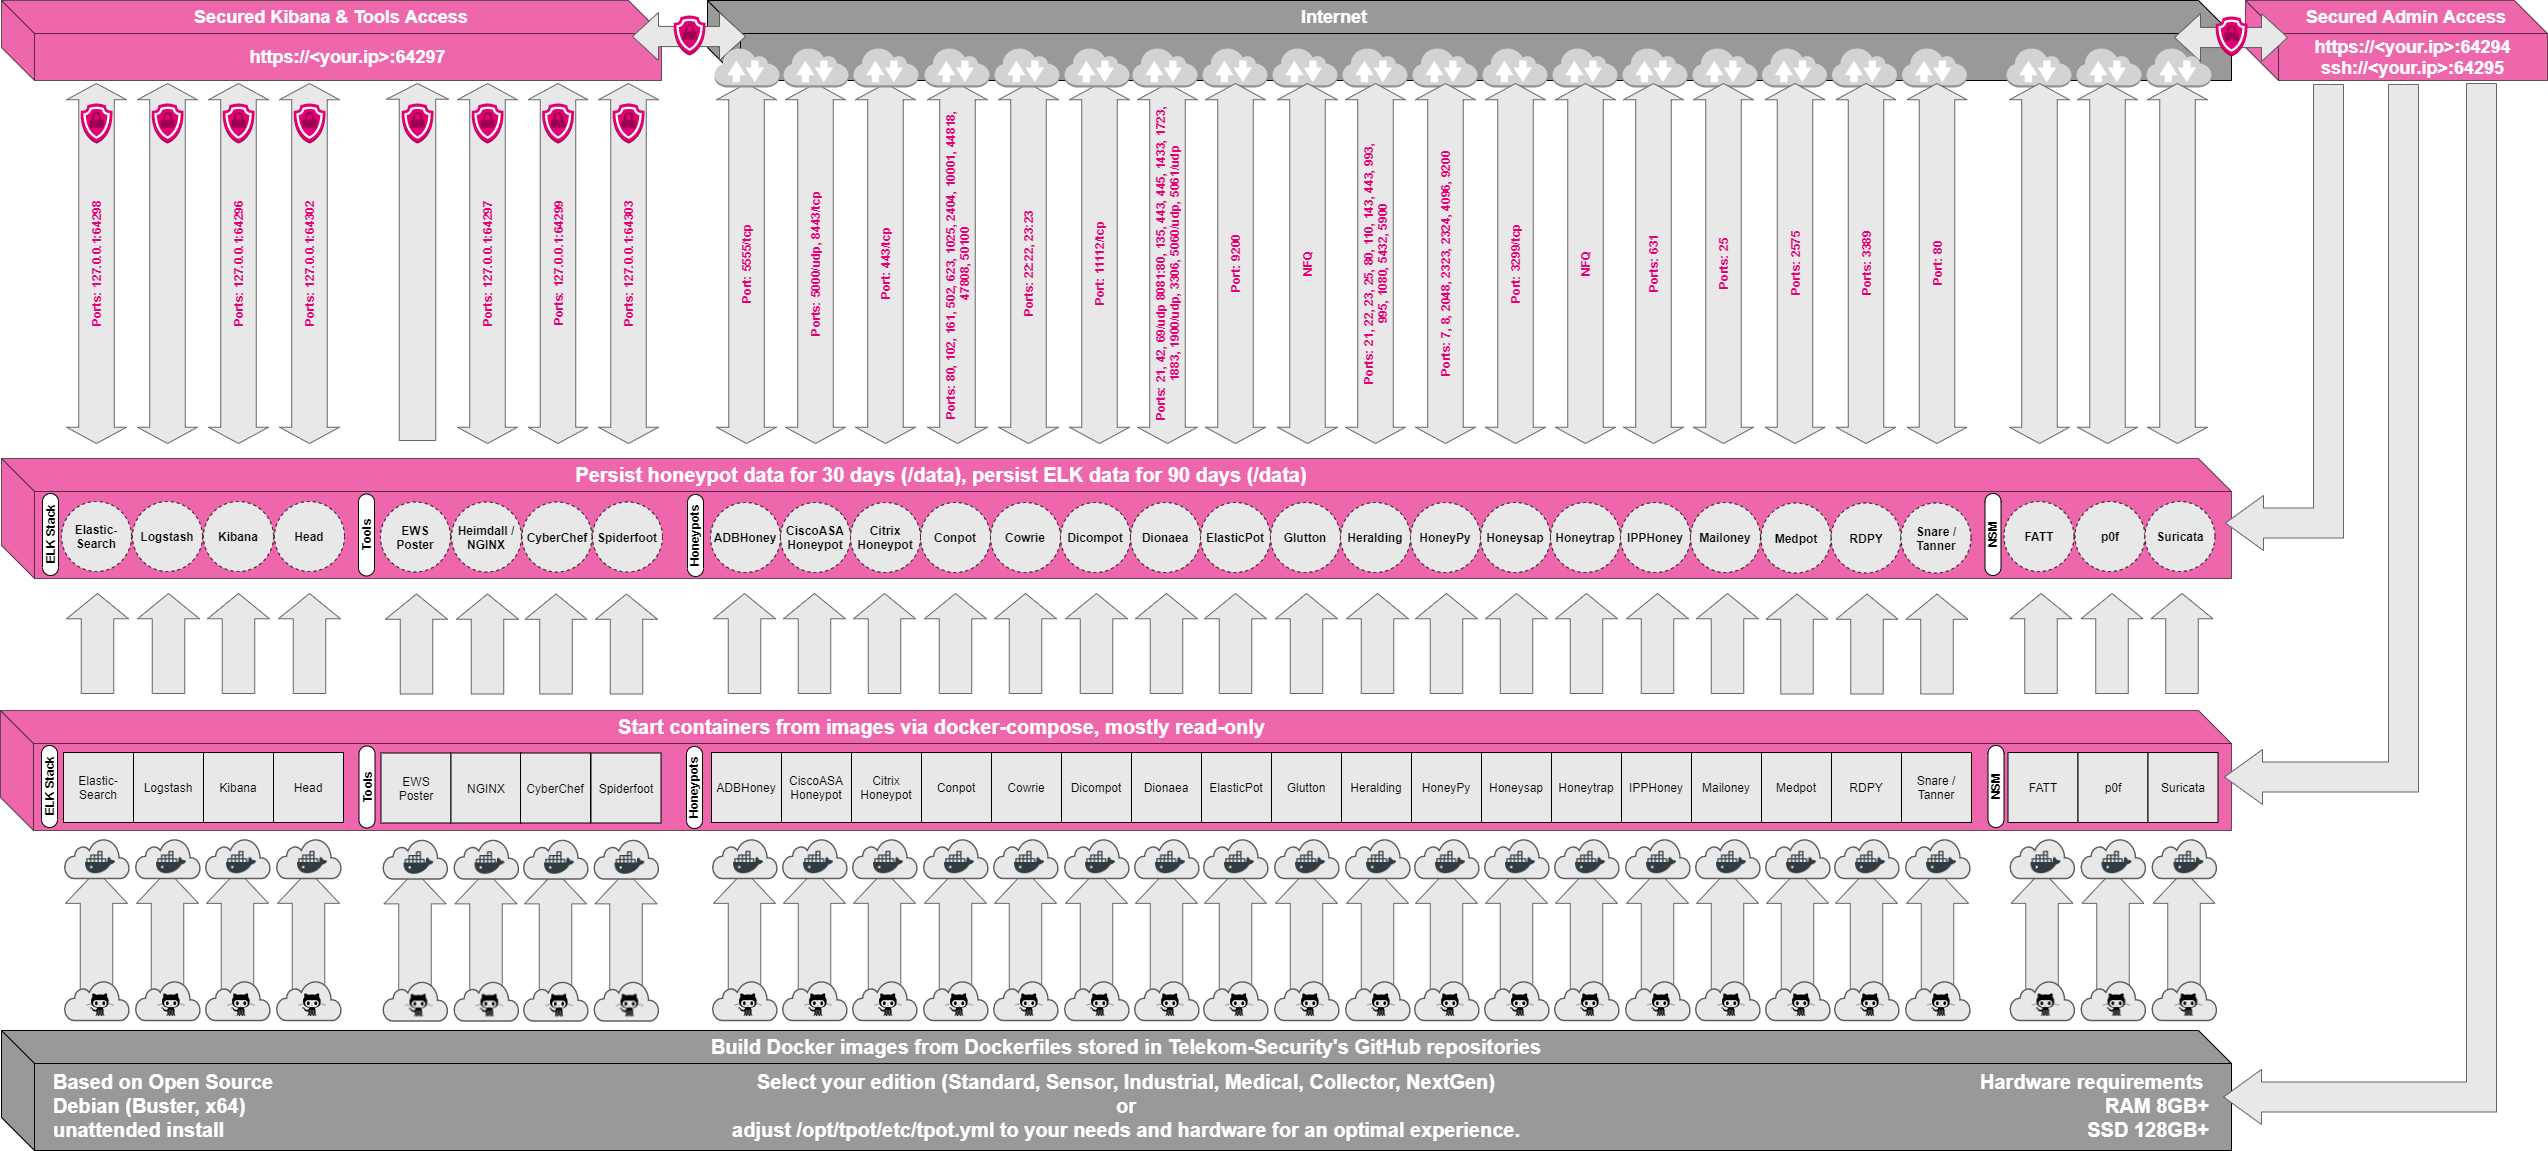
\includegraphics[width=\textwidth]{figures/architecture.png}
    \caption{}
    \label{fig:overview-tpot}
\end{sidewaysfigure}

\section{Data Analysis}

\begin{enumerate}
    \item Attack Profile
    \item Attack Source
    \item Attack Target
    \item Attack Frequency
    \item Attack Evolution
    \item Propagation of Attacks
    \item Attack Patterns
    \item Attack Root Cause Identification
    \item Attack Risk Assessment
    \item Exploit Detection
\end{enumerate}

\todo{übersicht tabelle}
\begin{table}[h]
    \centering
    \caption{}
    \begin{tabularx}{\linewidth}{l}
        \toprule
        \bottomrule
    \end{tabularx}
    \label{tab:overview-data-analysis}
\end{table}


\section{Results in HeiCloud}

\todo{verwendung von Grafiken, etc.}

\todo{show results}

\section{Summary}